%==============================================================
% Springer Requirements Engineering (RE) journal submission (English)
% Class: Springer Nature sn-jnl (numeric reference style, RE uses [1]-style)
% Double-blind (double-anonymous) version: author/affiliation are anonymized here.
% Real author/affiliation/declarations are in title_page.tex (submit separately).
%
% IMPORTANT (compile on Overleaf):
%   sn-jnl.cls / sn-basic.bst are NOT in Overleaf's base TeX Live. Create a new
%   project from the official "Springer Nature LaTeX Template" (Overleaf gallery),
%   then upload/replace with the files in this zip. See README_OVERLEAF.md.
%==============================================================
\documentclass[sn-mathphys-num]{sn-jnl}

\usepackage{graphicx}
\usepackage{multirow}
\usepackage{amsmath,amssymb,amsfonts}
\usepackage{booktabs}
\usepackage{tabularx}
\usepackage{array}
\usepackage{float}
\usepackage{rotating}
\usepackage{placeins}

\begin{document}

\title[Beyond Majority Vote]{Beyond Majority Vote: Improving Per-Requirement Quality Assessment via Good Outlier Recognition and Roundtable Consensus}

% ---- Double-blind: author information anonymized (real info in title_page.tex) ----
\author[1]{\fnm{Anonymous} \sur{Author}}
\affil[1]{\orgname{Anonymous Institution}}

\abstract{High-quality assessment of software requirements specifications is critical to project success. Although large language models (LLMs) show strong potential for automated requirements review, existing multi-agent collaboration methods often fall into a ``consensus fallacy'' in which agreement is equated with correctness. Majority voting or mean aggregation tends to suppress minority opinions---outliers---that may reveal deep, high-value defects. To overcome this limitation, we propose an outlier-aware multi-LLM collaboration workflow for per-requirement quality assessment. Heterogeneous models independently produce structured reviews along four quality dimensions (Understandable, Unambiguous, Correctness, Verifiable); a six-dimensional argument-quality vector then distinguishes ``good'' from ``bad'' outliers at the level of textual reasoning. On this basis, a Bayesian-inspired weighting scheme converts each model's demonstrated ability to capture high-value outliers into a fixed profile weight, which is combined with dynamic confidence in a per-item roundtable consensus. On the public PURE dataset with five heterogeneous LLMs, we observe structurally significant disagreement in requirements-quality judgments, especially for Verifiability. The proposed workflow penetrates numerical deviation, blocks unsupported hallucinations, and amplifies well-argued minority insights. Compared with single-model and equal-weight baselines, it does not chase absolute score agreement but substantially compresses redundant candidate defects and yields a compact, highly stable, higher-precision, and engineering-actionable team-level issue list, offering an alternative to the majority-vote paradigm for automated requirements quality assurance.}

\keywords{Requirements quality, Large language models, Multi-agent consensus, Disagreement and outliers, Requirements review}

\maketitle

\section{Introduction}\label{sec:introduction}
In the modern software engineering lifecycle, the quality of a Software Requirements Specification (SRS) directly determines the success of downstream architectural design, implementation, and testing. Traditional requirements quality assurance relies mainly on expert review or rule-based static analysis (e.g., requirements-smell detection); such approaches are labor-intensive and struggle to capture the semantic subtleties of natural-language requirements. As large language models (LLMs) have demonstrated strong natural-language understanding and reasoning abilities, researchers have increasingly explored their use in requirements engineering (RE) for automated drafting, defect classification, and quality review.

Although a single LLM (LLM-as-a-Judge) shows considerable promise for requirements quality assessment, its inherent biases, opaque internal reasoning, and occasional hallucinations make it difficult to provide robust diagnoses for complex industrial requirements. Consequently, research has shifted toward multi-agent collaboration and consensus mechanisms that introduce several heterogeneous LLMs for cross-validation or debate to compensate for the blind spots of any single model. However, existing multi-model aggregation methods---majority voting, simple mean aggregation, or multi-round roundtable discussion that merely seeks output agreement---implicitly rely on the assumption that ``convergence implies correctness'' (the consensus fallacy). In the highly subjective, reasoning-intensive task of requirements quality review, this assumption is flawed. When a model's score deviates sharply from the group median (i.e., triggers an outlier event), it does not necessarily indicate an error. The deviation may reflect a hallucinated or weakly evidenced ``bad outlier'', but it may equally reflect a ``good outlier'' in which the model has detected a hidden defect overlooked by the majority and can support it with sound reasoning. Naively converging to the majority or the median tends to erase these high-value minority insights.

To break the consensus fallacy in multi-model requirements review, we propose an \emph{outlier-aware consensus workflow} for per-requirement quality assessment. Our core idea is not to treat inter-model disagreement as random noise to be filtered out, but to convert it into structured reliability evidence that drives high-quality review. Concretely, heterogeneous models independently score each requirement on Understandability (U), Unambiguity (A), Correctness (C), and Verifiability (V), and output supporting evidence and rewrite suggestions; the framework then prescreens outlier events against the median and introduces a six-dimensional argument-quality vector---covering evidence sufficiency, rewrite executability, and related features---to distinguish good from bad outliers at the semantic-reasoning level. On this basis, we adopt a Bayesian-inspired reliability-updating view: a model's outlier behavior within the current document is accumulated into a model profile that yields a fixed prior weight for subsequent discussion; finally, in a per-item roundtable consensus, this fixed weight is combined with dynamic confidence so that a heterogeneous model team converges to a highly structured final issue list while preserving valuable disagreement.

To evaluate the effectiveness and engineering utility of the proposed framework, we conduct a rigorous within-subject empirical study on the public PURE requirements dataset with five mainstream heterogeneous LLMs. Through careful ablation against single-model review, an equal-weight aggregation baseline, and an unweighted roundtable, we examine the structure of initial disagreement, the discriminative power of argument-quality judgment, and the trade-off between defect recall and issue-list quality of the complete framework.

The main contributions of this paper are as follows:
\begin{itemize}
\item \textbf{Structural characterization of disagreement in multi-LLM requirements review.} We empirically show that models produce pronounced outlier judgments on complex defects, especially for Verifiability and Unambiguity, supporting the view that model disagreement is a high-value review signal rather than noise.
\item \textbf{Argument-quality-based good/bad outlier discrimination with Bayesian-inspired weighting.} We move automated requirements review from ``numerical statistical aggregation'' to ``textual reasoning validation'', dynamically extracting effective outlier evidence to anchor each model's true reliability in the current review task.
\item \textbf{A per-item roundtable consensus workflow fusing fixed weights and dynamic confidence.} Empirically, the workflow suppresses low-quality deviation and, without pursuing absolute score agreement, substantially compresses redundant candidate issues, producing a compact, highly stable, higher-precision, and engineering-actionable team-level defect list.
\end{itemize}

\section{Background and Related Work}\label{sec:related}
We review three areas most relevant to this study and contrast our work with the state of the art to position our contribution within empirical software engineering.

\subsection{Requirements quality assessment, defect classification, and LLMs in RE}
Requirements quality assessment is a foundational problem in RE and a long-standing focus of mainstream software engineering research~\cite{ref1}. Prior work discusses ``what constitutes high-quality requirements'', covering quality definitions, improvement techniques, and evaluation methods~\cite{ref2}, while also noting persistent conceptual fragmentation, inconsistent quality-attribute definitions, and a weak link between quality assessment and downstream development~\cite{ref3}. Montgomery et al.'s systematic mapping shows that requirements-quality research is already substantial yet dispersed in objects, attributes, and evaluation methods~\cite{ref2}; Frattini et al. propose a harmonized theory arguing that requirements quality must be connected to actual downstream effects rather than remaining at the level of normative rules~\cite{ref3}; Femmer and Vogelsang, from a ``quality in use'' perspective, argue that requirements quality is not merely textual conformance but real usability in understanding, implementation, and verification~\cite{ref4}. For our purposes, these works establish that requirements review must attend to both textual properties and engineering usability. At the level of concrete defect identification, several actionable paths exist: Femmer et al. propose requirements smells, treating vagueness, redundancy, and unclear phrasing as lightweight quality defects for rapid assurance~\cite{ref5}; Lucassen et al. propose the Quality User Story framework, turning quality into checkable criteria~\cite{ref6}; ICSE-community work further analyzes requirements-quality improvement and evolution through structured patterns and quality snapshots~\cite{ref7,ref8}. These studies show that requirements quality is not an unactionable abstraction but can be identified via rules, patterns, or metrics. However, most work focuses on single-document rule checking, static smell detection, or quality-evolution analysis, treating automated assessment as a single-method or single-tool problem; it rarely addresses how to handle pronounced disagreement among multiple reviewers on the same requirement item, and does not organize such disagreement as input to subsequent weight modeling and team consensus.

The application of LLMs in RE has expanded from simple text generation to complex quality-assurance tasks. Krishna et al. use GPT-4 to evaluate the PURE dataset~\cite{ref9} and show that LLMs approach junior-engineer competence in drafting and reviewing SRS~\cite{ref10}; Zadenoori et al. summarize broad attempts to handle ambiguity (Unambiguity) and testability (Verifiability) in natural-language requirements~\cite{ref11}. Nevertheless, LLM-based requirements review still has clear limitations: for example, Oriol et al.'s recent MAD-RE study explores multi-agent debate (MAD) for requirements classification~\cite{ref12} but essentially treats models as label-emitting ``black boxes'', focusing on category agreement while neglecting the core of requirements review---deep argumentation over the semantics of disagreement, i.e., aligning the logical chain of ``requirement ambiguity (evidence)'' and ``rewrite strategy''. Moreover, the prevailing ``LLM-as-a-Judge'' paradigm~\cite{ref13,ref14} often suffers from calibration failure. We differ in that we not only require Likert scores~\cite{ref10} but also explicitly measure the textual evidence of model outputs via a six-dimensional argument-quality vector, thereby addressing the lack of a per-requirement, evidence-grounded conflict-resolution mechanism in existing RE-LLM research that otherwise tends to settle into ``mediocre consensus'' on complex industrial requirements.

\subsection{Multi-LLM collaboration and consensus}
In parallel with single-model judges, research on multi-LLM collaboration, discussion, and consensus assumes that communication, questioning, and persuasion among models can expose reasoning blind spots and, through multi-round interaction, form more robust collective judgments. To counter single-model bias, multi-agent dialogue and writing frameworks have been proposed~\cite{ref15,ref16,ref17}. Among them, RECONCILE~\cite{ref18} is a landmark work introducing multi-round round-table conferencing and confidence-weighted voting to improve LLM reasoning consistency. Kaesberg et al. further discuss the merits of ``voting'' versus ``consensus'' across tasks~\cite{ref19}; Exchange-of-Thought emphasizes the role of cross-model communication in complex problem solving~\cite{ref20}; and multi-agent debate work argues that divergent thinking is not noise but a key resource for better reasoning~\cite{ref16}. Collectively, these works motivate an important shift: in multi-model systems, differences and conflicts need not be immediately smoothed away; a carefully designed interaction process may itself be the prerequisite for better team decisions~\cite{ref16,ref20}.

For our purposes, these works provide mechanistic foundations rather than directly reusable solutions. Existing multi-LLM collaboration mostly targets general reasoning, question answering, or generic text evaluation, and rarely descends to artifact-centric, issue-type-oriented tasks such as requirements quality review. Their objects of discussion are typically a single answer or judgment, whereas our goal is a structured issue list over a single requirement item along U/A/C/V, retaining both evidence and rewrites. Although prior work distinguishes voting from consensus~\cite{ref19}, which decision mechanism can both preserve the value of disagreement and yield engineering-actionable output in requirements review remains under-studied. Thus, the multi-agent discussion literature inspires our ``fixed weight + dynamic confidence'' per-item roundtable consensus but does not directly cover the requirements-quality review setting.

\subsection{Disagreement handling and weighted aggregation}
Handling disagreement is a classic problem in multi-annotator aggregation. Dawid and Skene first systematically estimated observer error rates from multiple judgments~\cite{ref21}; Whitehill et al. studied optimal integration of labels from annotators of unknown expertise~\cite{ref22}. Aroyo and Welty's ``Crowd Truth'' critiques the myth of a single correct truth, arguing that disagreement often carries task complexity~\cite{ref23}. In model ensembling, Hovy et al.'s MACE advances annotator-ability modeling into a probabilistic-graphical framework that infers reliability from labeling disagreement~\cite{ref24}. A common premise is that differences among judgment sources should not be blindly averaged but explicitly modeled as ``who is more trustworthy''. In this sense, our construction of model profiles and fixed weights from good/bad outliers has a clear methodological kinship with reliability-aware weighting.

However, our goal differs from classic reliability-aware aggregation. Classic annotator aggregation usually assumes recovery of a latent truth, so disagreement is treated as uncertainty to be explained away. In contrast, recent ``learning from disagreement'' research argues that in subjective or multi-criteria tasks, disagreement itself may carry valuable information and should not be compressed into a single label~\cite{ref25}; work on instruction-tuned models likewise shows that treating multiple LLMs as a ``model crowd'' is meaningful, since different models exhibit systematic label variation and the aggregation method markedly affects quality~\cite{ref26}. We push this further: we do not treat outlier scores as errors but ask which outliers are high-value dissent and which are merely low-quality deviation; nor do we treat weights as static priors---weights derive from the argument quality of outlier events. As Aroyo et al.~\cite{ref23} note, pure consensus is often mediocre. Rather than statistically penalizing outliers, we semantically validate them: through a six-dimensional feature vector we identify ``good outliers'' that deviate from the median yet exhibit high argument quality. This move from ``label statistics'' to ``textual reasoning validation'' lets us surface requirement defects overlooked by the majority.

\section{Problem Statement and Research Questions}\label{sec:problem}

\subsection{Problem statement}
Unlike document-level evaluation, our analysis granularity is fixed at per-requirement quality assessment within a single requirements document: each requirement is an independent review unit. Given an input set of requirement items, several heterogeneous LLMs (reviewers) score each item along Understandability (U), Unambiguity (A), Correctness (C), and Verifiability (V) on a Likert 1--5 scale, and provide confidence, evidence spans, and rewrite suggestions. The final output goes beyond document-level score aggregation, providing for each requirement a team-level diagnosis containing item id, issue type, evidence span, suggested rewrite, and influence.

In multi-LLM requirements review, models often disagree on the same item and dimension. Such disagreement is not incidental noise but a structural phenomenon arising from differences in architecture, training data, alignment, reasoning style, and understanding of semantic boundaries. Majority voting or mean aggregation implicitly assumes that judgments closer to the group center are more reliable and that deviations are more suspect. In requirements review this assumption is inadequate: a deviating score may stem from hallucination, misunderstanding, or weak evidence, but it may also indicate that the model has captured a hidden defect missed by others. An ``outlier'' is therefore not necessarily an error; the key question is whether a deviating judgment carries review value.

From an uncertainty-modeling viewpoint, multi-LLM requirements review is a multi-observer inference problem. The true defect status of an item/dimension is not directly observable and can only be inferred from the scores, confidences, evidence, and rewrites of multiple models---each a noisy observation carrying model preferences, capability differences, and hallucination risk. Aggregation is thus not mere averaging but, absent direct ground truth, updating each model's review reliability from its output quality and outlier behavior in the current document, and then inferring whether a candidate defect should be retained as a team-level conclusion.

Accordingly, we treat good and bad outliers as observational evidence for reliability updating: if a model repeatedly produces deviations that are well evidenced, dimension-aligned, and executable, these events raise its subsequent influence; conversely, deviations that lack evidence, mismatch the dimension, or are non-actionable lower it. We do not assume equal reliability across models, nor rank them statically by general benchmarks; instead we build a task-internal, document-internal model profile from good/bad-outlier behavior, and apply a conservative, Bayesian-style reliability update to derive the fixed model weights used in the roundtable stage. This distinguishes our approach from single-model review, from simple equal-weight aggregation, and from consensus-only multi-agent discussion that treats disagreement as noise to eliminate.

In summary, our problem is: in per-requirement U/A/C/V quality assessment, how to convert structured multi-LLM disagreement from raw score deviation into interpretable reliability evidence, and use that evidence to drive weight updating and per-item roundtable consensus. To this end we build a complete decision chain from initial-disagreement identification, outlier-quality discrimination, model profiling and posterior-style weighting, to a team-level issue list produced by fusing fixed weights and dynamic confidence---avoiding the consensus fallacy while suppressing low-quality deviation and preserving high-value minority opinions.

\subsection{Research questions}
Our three research questions follow three logical layers---individual differences, workflow effect and trade-off, and variation across documents/dimensions:
\begin{description}
\item[RQ1.] \emph{How do individual LLMs differ in identifying per-requirement quality issues in software requirements?} We analyze whether different LLMs exhibit systematic differences in score distribution, evidence use, issue-type identification, dimension sensitivity, and outlier behavior along U/A/C/V, to characterize whether observable structural disagreement exists among initial judgments.
\item[RQ2.] \emph{How does the proposed outlier-aware consensus workflow compare with individual LLMs and aggregation baselines in producing per-requirement quality issue lists?} We assess ground-truth alignment, issue-list size, evidence support, set convergence, and human-review usability, without assuming the method dominates on every metric.
\item[RQ3.] \emph{How does the performance of the consensus workflow vary across requirements documents and quality dimensions?} We examine how performance changes with document size, defect density, domain context, and the U/A/C/V dimensions, to identify the method's applicability boundaries.
\end{description}

\section{Methodology}\label{sec:method}
We build an automated requirements-quality-assessment framework that fuses multiple LLMs with a dynamic roundtable consensus. Within a single document and at per-requirement granularity, it organizes the quality judgments, evidence, and rewrite suggestions of heterogeneous LLMs into an interpretable, reproducible team-level issue list. Let the requirement set be $\mathcal{I}=\{1,\dots,n\}$ and the dimension set $\mathcal{D}=\{U,A,C,V\}$. For any model $r\in\mathcal{R}$, item $i\in\mathcal{I}$, and dimension $d\in\mathcal{D}$, the model outputs a Likert $1..5$ score $s_{r,i,d}$ together with confidence, an evidence span, and a rewrite suggestion. The pipeline comprises seven stages: (1) structured per-requirement scoring; (2) median-based outlier prescreening; (3) argument-quality vector scoring; (4) good/bad outlier discrimination; (5) model profiling and weight construction; (6) per-item roundtable consensus fusing fixed weights and dynamic confidence; and (7) final issue-list extraction.

To strengthen statistical interpretability, we view the weighting process through Bayesian reliability updating: good/bad outliers within the current document act as evidence supporting or weakening reliability; each model receives a uniform, conservative prior, which is updated by observed good/bad outliers into a posterior reliability that becomes the fixed roundtable weight. This interpretation does not alter the outlier definition, argument-quality vector, or roundtable procedure; it justifies why good outliers should be up-weighted and bad outliers down-weighted.

\begin{figure}[t]
\centering
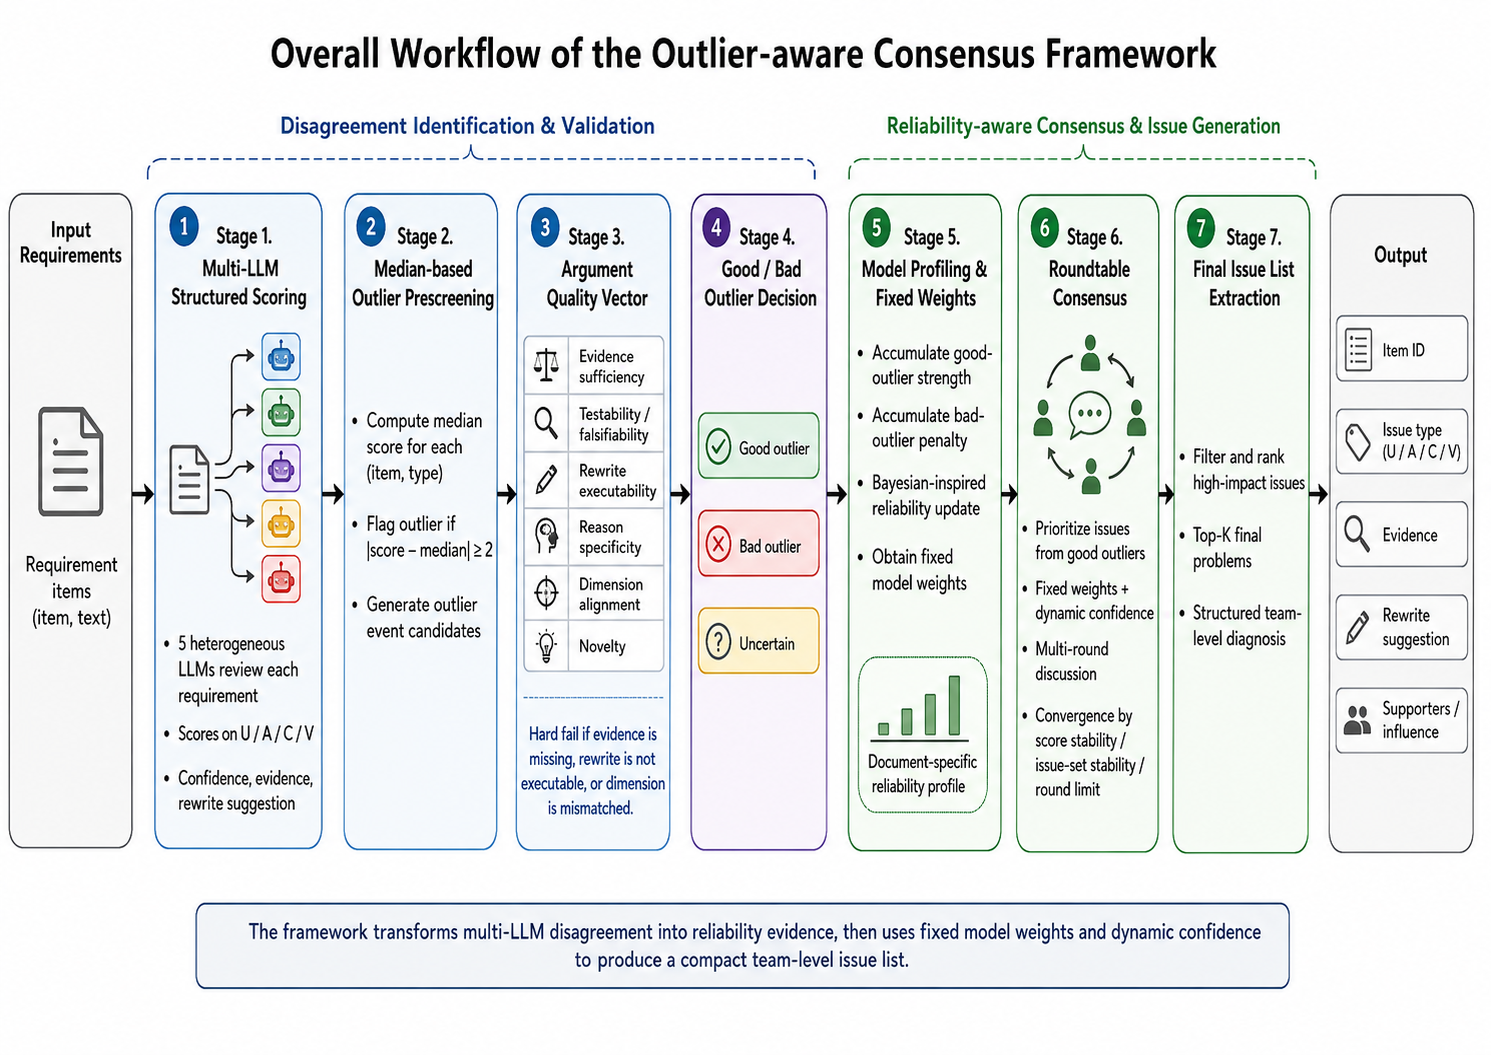
\includegraphics[width=\linewidth]{figures/fig1_overall_workflow.png}
\caption{Overall workflow of the proposed outlier-aware multi-LLM consensus framework.}
\label{fig:overall_workflow}
\end{figure}

\subsection{Stage 1: Structured per-requirement scoring}
Because the granularity is strictly per-requirement, we input a requirements table with item id and text, and treat several heterogeneous LLMs as virtual reviewers. For each requirement, every model independently infers along each dimension on a Likert $1..5$ scale, and must output the four-dimensional scores, an initial confidence, the corresponding evidence span, and an atomic, unambiguous, executable rewrite suggestion. This stage (i) unifies model opinions into the same dimensional protocol and numeric range so that outlier detection is comparable, and (ii) explicitly retains evidence and rewrites---not only numeric scores---providing auditable semantic material for later argument-quality judgment and roundtable discussion.

\subsection{Stage 2: Automatic outlier prescreening}
Multi-LLM scores often disagree strongly. This stage identifies ``outlier events'' that deviate sharply from the group consensus as the focus for deeper review. To remove single-model bias, we use the group median as the consistency baseline. For each item and dimension we construct the median baseline over all reviewers:
\begin{equation}
\tilde{s}_{i,d} = \operatorname{median}_{r \in R}\!\left(s_{r,i,d}\right)
\label{eq:median}
\end{equation}
and compute the deviation and absolute deviation of each score:
\begin{equation}
\mathrm{deviation}_{r,i,d} = s_{r,i,d} - \tilde{s}_{i,d}
\label{eq:deviation}
\end{equation}
\begin{equation}
\mathrm{abs\_deviation}_{r,i,d} = \left| \mathrm{deviation}_{r,i,d} \right|
\label{eq:absdev}
\end{equation}
With an outlier sensitivity threshold $\theta=2$, a triple $(r,i,d)$ triggers an outlier event when $\mathrm{abs\_deviation}_{r,i,d}\ge\theta$. The output is a set of outlier events forming the candidate pool for argument-quality assessment. The goal here is not to treat deviating judgments as errors, but to build a ``needs-focused-review'' candidate set.

\subsection{Stage 3: Argument-quality vector scoring}
An outlier is not necessarily an error (``bad outlier''); it may be a model detecting a hidden defect with high-quality argumentation (``good outlier''). This stage quantifies the textual output of each outlier event via six features: evidence sufficiency ($E$), falsifiability/testability ($F$), rewrite executability ($R$), rationale specificity ($S$), dimension fit ($T$), and novelty ($D$). Each sub-item is scored on a discrete scale, and the normalized argument-quality score is:
\begin{equation}
Q_{r,i,d} = \frac{1}{6}\left(
\frac{q^{E}_{r,i,d}}{2} + \frac{q^{F}_{r,i,d}}{2} + \frac{q^{R}_{r,i,d}}{2}
+ \frac{q^{S}_{r,i,d}}{2} + \frac{q^{T}_{r,i,d}}{2} + \frac{q^{D}_{r,i,d}}{2}
\right) \in [0,1]
\label{eq:Q}
\end{equation}
We also enforce a strict ``hard-fail'' rule: if evidence sufficiency, rewrite executability, or dimension fit is $0$, the event is directly classified as a bad outlier, regardless of other sub-items.

\subsection{Stage 4: Good/bad outlier discrimination}
Without changing the outlier definition, we set empirical thresholds as automatic decision boundaries:
\begin{equation}
\mathrm{decision}_{r,i,d} =
\begin{cases}
\mathit{bad}, & \text{if } \mathit{hard\_fail} = \mathit{true}\ \text{or}\ Q_{r,i,d} \le \tau_{bad} \\
\mathit{good}, & \text{if } \mathit{hard\_fail} = \mathit{false}\ \text{and}\ Q_{r,i,d} \ge \tau_{good} \\
\mathit{uncertain}, & \text{otherwise}
\end{cases}
\label{eq:decision}
\end{equation}
with $\tau_{good}=0.60$ and $\tau_{bad}=0.30$; grey-zone events are labeled uncertain and only optionally overwritten by ``prescreening + light human confirmation''. This yields a labeled decision table that supervises weight learning, and reframes outlier information from ``anomalies'' to ``dissenting samples of differing review value''.

\subsection{Stage 5: Model profiling and weight construction}
Unlike the equal-weight voting of classic ensembles, we assign each model a global fixed weight according to its ability to handle outlier events---reflecting relative review reliability under the current document and task, not a general capability ranking. We accumulate event-level judgments into a model profile and define each model's positive contribution (good-outlier strength $G_r$) and negative penalty (bad-outlier strength $B_r$):
\begin{equation}
G_r = \sum_{i,d} \mathbf{1}\!\left[\mathrm{decision}_{r,i,d} = \mathit{good}\right]
\times \mathrm{abs\_deviation}_{r,i,d} \times Q_{r,i,d}
\label{eq:Gr}
\end{equation}
\begin{equation}
B_r = \sum_{i,d} \mathbf{1}\!\left[\mathrm{decision}_{r,i,d} = \mathit{bad}\right]
\times \mathrm{abs\_deviation}_{r,i,d} \times \left(1 - Q_{r,i,d}\right)
\label{eq:Br}
\end{equation}
To prevent one or two outliers from dominating in small samples, we compute a smoothed document evidence score with constant $\kappa$:
\begin{equation}
\mathrm{score}_{doc}(r) = \frac{G_r - \lambda B_r}{\kappa + n_{good}(r) + n_{bad}(r)}
\label{eq:scoredoc}
\end{equation}
where $\kappa>0$ is a conservative prior-sample-size term, fixed to $\kappa=3.0$ so that when only 1--2 effective outliers occur, weights adjust mildly rather than being dominated by a single event. As we introduce no separate cross-document calibration set, all models receive a uniform prior $w_{prior}(r)=1/|\mathcal{R}|$ before observing effective outlier evidence. We define the document's total effective outlier evidence and evidence strength as:
\begin{equation}
T_{doc} = \sum_{r \in \mathcal{R}} \left(G_r + B_r\right)
\label{eq:Tdoc}
\end{equation}
\begin{equation}
\rho_{doc} = \frac{T_{doc}}{T_{doc} + \eta}
\label{eq:rhodoc}
\end{equation}
where the document-level prior strength $\eta$ controls how far current-document evidence updates the default prior, fixed to $\eta=4.0$. The document-induced softmax weight and the final fixed weight for the per-item roundtable are:
\begin{equation}
w_{doc}(r) = \frac{\exp\!\left(\beta \cdot \mathrm{score\_doc}(r)\right)}
{\sum_{j \in \mathcal{R}} \exp\!\left(\beta \cdot \mathrm{score\_doc}(j)\right)}
\label{eq:wdoc}
\end{equation}
\begin{equation}
w_r = (1 - \rho_{doc}) \cdot w_{prior}(r) + \rho_{doc} \cdot w_{doc}(r)
\label{eq:wr}
\end{equation}
The fixed weight is not a standalone output but a prior-influence term in the roundtable; its actual contribution is evaluated in the ablation against the unweighted roundtable.

\subsection{Stage 6: Per-item roundtable consensus fusing fixed weights and dynamic confidence}
Inspired by RECONCILE, this stage runs multi-round interaction within a single requirement under three fixed constraints: (i) the roundtable never discusses ``outliers'' explicitly---outliers are used only for prior weighting; (ii) model weights stay fixed throughout; (iii) each model's confidence, representing its current certainty, is updated dynamically across rounds. For candidate construction we prioritize $(i,d)$ pairs corresponding to good outliers, falling back to the full issue set when insufficient. For each model, item, and dimension we define an influence, and aggregate the influences of supporting models into the team score of an issue:
\begin{equation}
\mathrm{influence}_{r,i,d} = w_r \times \mathrm{conf}_{r,i,d}
\label{eq:influence}
\end{equation}
\begin{equation}
S_{issue}(i,d) = \sum_{r \in \mathcal{R}^{+}_{i,d}} \mathrm{influence}_{r,i,d}
\label{eq:Sissue}
\end{equation}
where $\mathcal{R}^{+}_{i,d}$ is the set of models supporting an issue on $(i,d)$. Each round ranks candidate issues by team score. Termination uses three criteria: score convergence, issue-set convergence (measured by set overlap), and a fixed round cap.

\subsection{Stage 7: Final issue-list extraction}
Finally, from the team scores, evidence spans, and rewrite suggestions after consensus, we apply a selection confidence threshold to extract the final high-quality issue set:
\begin{equation}
\mathit{final\_problems} = \left\{ (i,d) \;\middle|\; S_{issue}(i,d) \ge \theta \right\}
\label{eq:final}
\end{equation}
Qualifying issues are ranked in descending order, and the Top-$K$ (e.g., 10) most influential defects form a highly structured team-level conclusion, standardized as: item id, issue type (U/A/C/V), evidence span, suggested rewrite, and supporters/influence.

\section{Experimental Design}\label{sec:experiment}
This section describes the empirical study evaluating the proposed multi-LLM requirements-review framework. Following the three RQs, the design proceeds from shallow to deep: first characterizing initial-scoring disagreement among heterogeneous LLMs (RQ1); then, via strict control variables and ablation baselines, evaluating the complete consensus workflow and its internal mechanisms in issue-list generation (RQ2); and finally examining generalization and performance variation across document characteristics and quality dimensions (RQ3).

\subsection{Experimental objectives and evaluation unit}
The experimental unit is strictly per-requirement evaluation within a single document. For each requirement, the system judges along U, A, C, and V; hence the minimal evaluation unit is the pair $(item,type)$ with $type\in\{U,A,C,V\}$. We evaluate not only numeric scoring but, more importantly, whether the system can produce a structured team-level diagnosis containing evidence spans and rewrite suggestions.

\subsection{Subjects and datasets}
\subsubsection{Evaluation subjects (heterogeneous LLMs)}
We select five mainstream LLMs with differing underlying architectures as virtual reviewers: DeepSeek-Reasoner, Qwen-plus, GPT-5.1, Kimi-k2-0905-preview, and GLM-5. This heterogeneous design realistically simulates the differing perspectives of an expert review team arising from different background knowledge, training corpora, and reasoning preferences, providing sufficient material for disagreement handling.

\subsubsection{Datasets}\label{sec:datasets}
We use PURE (PUblic REquirements dataset), widely used in empirical software engineering, which contains SRS documents from real industrial and open-source projects. By stratified sampling we select 10 documents covering different domains and sizes (from tens to hundreds of requirements) so that conclusions do not depend on a single context. The subset contains 978 requirement items and 3{,}912 $(item,type)$ evaluation units. PURE preserves real ambiguity, redundancy, and logical inconsistency, and parses into a uniform $(item, text)$ structure well suited to our fine-grained analysis.

\begin{table}[!ht]
\centering
\caption{Dataset and ground-truth summary.}
\label{tab:dataset_gt_summary}
\small
\begin{tabular}{lccccc}
\toprule
\textbf{Scope} & \textbf{Docs} & \textbf{Req. items} & \textbf{Dimensions} & \textbf{Units} & \textbf{GT positives} \\
\midrule
PURE subset & 10 & 978 & U/A/C/V & 3,912 & 240 (6.13\%) \\
\bottomrule
\end{tabular}

\vspace{0.6em}

\begin{tabular}{lccccc}
\toprule
\textbf{GT distribution} & \textbf{U} & \textbf{A} & \textbf{C} & \textbf{V} & \textbf{Total} \\
\midrule
Positive units & 44 & 135 & 4 & 57 & 240 \\
Positive rate & 4.50\% & 13.80\% & 0.41\% & 5.83\% & 6.13\% \\
\bottomrule
\end{tabular}

\par\vspace{0.4em}
{\footnotesize \textit{Note.} The evaluation unit is an $(item,type)$ pair, where $type \in \{U,A,C,V\}$ denotes Understandable, Unambiguous, Correctness, and Verifiable, respectively. Ground-truth labels are binary: $1$ indicates a quality issue in the corresponding dimension, $0$ otherwise. The final ground truth was built from two independent expert annotations, with disagreements resolved by a third senior adjudicator.\par}
\end{table}


\subsection{Treatments and baselines}\label{sec:treatments}
To answer RQ2 and isolate the contribution of each module, each document is evaluated in parallel under four treatments:
\begin{itemize}
\item \textbf{Single-LLM}: each of the five LLMs independently performs four-dimensional scoring and issue output, serving as the per-model lower bound.
\item \textbf{Equal-Weight Aggregation}: after independent scoring, issue scores are aggregated with equal weights, without argument-quality discrimination or outlier weighting, measuring the gain from merely adding models.
\item \textbf{Roundtable No Weighting}: retains multi-round dynamic confidence and roundtable discussion but removes the Bayesian update weights, so all models participate with equal influence.
\item \textbf{Full Method}: the complete decision chain of structured scoring $\to$ outlier-quality discrimination $\to$ evidence-driven posterior weighting $\to$ dynamic-confidence roundtable consensus.
\end{itemize}
The ablation logic is: Full Method vs.\ Roundtable No Weighting isolates the ``evidence-driven fixed weights''; Roundtable No Weighting vs.\ Equal-Weight Aggregation isolates the ``roundtable discussion mechanism''; Full Method vs.\ Single-LLM measures the overall gain over single-model review.

\begin{table}[!ht]
\centering
\caption{Treatments, baselines, and ablation settings.}
\label{tab:treatments_baselines}
\scriptsize
\setlength{\tabcolsep}{4pt}
\renewcommand{\arraystretch}{1.2}
\begin{tabularx}{\textwidth}{p{1.6cm} X p{1.5cm} p{1.5cm} p{1.7cm} X}
\toprule
\textbf{Treatment} &
\textbf{Input and aggregation} &
\textbf{Outlier-quality validation} &
\textbf{Fixed model weights} &
\textbf{Roundtable discussion} &
\textbf{Purpose in evaluation} \\
\midrule
\textbf{Single-LLM} &
Each LLM independently produces U/A/C/V scores, confidence, evidence, and rewrite suggestions per requirement; no cross-model aggregation. &
No & No & No &
Estimates the standalone capability of individual LLM reviewers; lower-bound reference for multi-LLM collaboration. \\
\midrule
\textbf{Equal-Weight Aggregation} &
All LLMs share the same round-0 structured outputs; candidate issue scores are aggregated under equal model influence. &
No & No; all models equal. & No &
Tests whether simply combining LLMs improves issue-list generation without disagreement validation or interaction. \\
\midrule
\textbf{Roundtable No Weighting} &
Same round-0 outputs and candidate issues; models take part in multi-round discussion. &
No good/bad validation for weighting. & No; equal influence. & Yes; dynamic confidence updated across rounds. &
Isolates the contribution of roundtable discussion while removing reliability-aware fixed weights. \\
\midrule
\textbf{Full Method} &
Complete structured output (scores, confidence, evidence, rewrites). &
Yes; argument-quality vector and hard-fail rules. & Yes; document-specific weights from good/bad-outlier evidence. & Yes; fixed weights combined with dynamic confidence. &
Evaluates the complete outlier-aware consensus workflow (validation, profiling, roundtable extraction). \\
\bottomrule
\end{tabularx}

\par\vspace{0.4em}
{\footnotesize \textit{Note.} All treatments are evaluated on the same requirement documents and share the same initial round-0 LLM outputs whenever applicable. This paired design controls for stochastic variation in LLM generation and isolates the effects of equal aggregation, roundtable discussion, and reliability-aware fixed weighting.\par}
\end{table}


\subsection{Metrics and ground truth}\label{sec:metrics}
To evaluate final issue-list quality we build ground truth (GT) by expert cross-blind annotation. Two experts with several years of RE experience independently annotate each $(item,type)$ pair for defect presence; disagreements are arbitrated by a third senior expert. Inter-annotator agreement is reported with Cohen's Kappa or Krippendorff's $\alpha$. Per RQ: RQ1 uses ordinal Krippendorff's $\alpha$ for initial-score agreement and the frequency/distribution of outlier events; RQ2 computes the normalized argument-quality score $Q$ and the share of events triggering ``hard fail'' (missing evidence, dimension mismatch, or non-executable rewrite); RQ3, given the severe class imbalance across the four defect types, adopts Macro-F1 as the core metric, and also reports Macro-Precision, Macro-Recall, and the issue-set Jaccard similarity between adjacent roundtable rounds.

\subsection{Control variables and reproducibility}
To minimize internal-validity threats we apply strict reproducibility controls: (1) \textbf{Shared initial state}: all aggregation and roundtable baselines share the same batch of round-0 model outputs (initial scores, confidence, evidence), eliminating input inconsistency due to LLM API sampling randomness; (2) \textbf{Unified parameters}: all documents share fixed hyperparameters---outlier threshold $\theta=2$; good/bad thresholds $\tau_{good}=0.60$, $\tau_{bad}=0.30$; Bayesian smoothing $\kappa=3.0$, $\eta=4.0$; softmax penalty $\lambda=1.5$; maximum roundtable rounds $=2$; (3) \textbf{Robustness control}: an exponential-backoff retry mechanism is deployed; if a model repeatedly fails on a specific item, it is isolated (skipped) for that case while the others continue, testing robustness under ``missing review members''.

\subsection{Data analysis methods}\label{sec:analysis}
Statistical analysis is blocked by document to avoid Simpson's paradox from directly mixing heterogeneous items. We use $\alpha=0.05$ as the significance level and report non-parametric effect sizes alongside significance. For RQ1 (disagreement structure) we use a Friedman test on whether the frequency of strong outlier events differs across U/A/C/V; for RQ2 (discrimination) a Mann--Whitney U test compares good vs.\ bad outliers on $Q$ and sub-dimensions, with Cliff's $\delta$ effect sizes; for RQ3 (performance and ablation), since each document is evaluated under all four treatments, a global Friedman test compares Macro-F1 and, if significant, Holm--Bonferroni-corrected pairwise comparisons follow, together with Jaccard curves and score-fluctuation decay plots to visualize convergence.

\section{Results}\label{sec:results}
All results are based on ground truth (GT), the current multi-model outputs, and document-level statistics. To keep the Full-Method diagnosis and treatment-level comparison over the same coverage, we use 10 shared requirements documents as a unified analysis scope.

\subsection{RQ1: How do individual LLMs differ in identifying per-requirement quality issues?}
To characterize initial-judgment differences, we first compute ordinal Krippendorff's $\alpha$ on the round-0 score matrix (all documents and models using the same prompt, parser, and thresholds, so that treatments share the same starting point). Overall agreement across all 10 documents, 978 requirements, and 3{,}912 $(item,type)$ units is $0.4232$, indicating limited convergence at initial scoring. Decomposed by dimension, the $\alpha$ for U/A/C/V is $0.0258$, $-0.0377$, $0.1202$, and $0.0526$, respectively, showing that at the fine-grained U/A/C/V level models fail to reach stable agreement---some dimensions even fall below chance.

Score distributions also differ markedly by dimension. The medians of U and C are both $3$, while A and V are $2$; the means are U$=2.6279$, A$=2.0602$, C$=2.8605$, and V$=1.7030$. V has the lowest mean, whereas C is the highest---so the model population is more prone to flagging low ``problematic'' scores on verifiability while being more conservative on correctness.

At outlier prescreening ($|score-median|\ge 2$), the distribution shows pronounced dimensional clustering rather than random noise. Across the 10 documents we identify 60 outlier events. By dimension, V triggers 42 outliers ($70.00\%$), while U, A, and C have only 7 ($11.67\%$), 6 ($10.00\%$), and 5 ($8.33\%$). Normalizing by within-document outlier rate, differences remain significant: V has the highest average rate ($1.26\%$), well above U ($0.20\%$), A ($0.15\%$), and C ($0.15\%$); a Kruskal--Wallis test confirms a statistically significant difference in within-document outlier rates across the four dimensions ($H=10.7601$, $\mathrm{df}=3$, $p=0.0131$).

\begin{figure}[t]
\centering
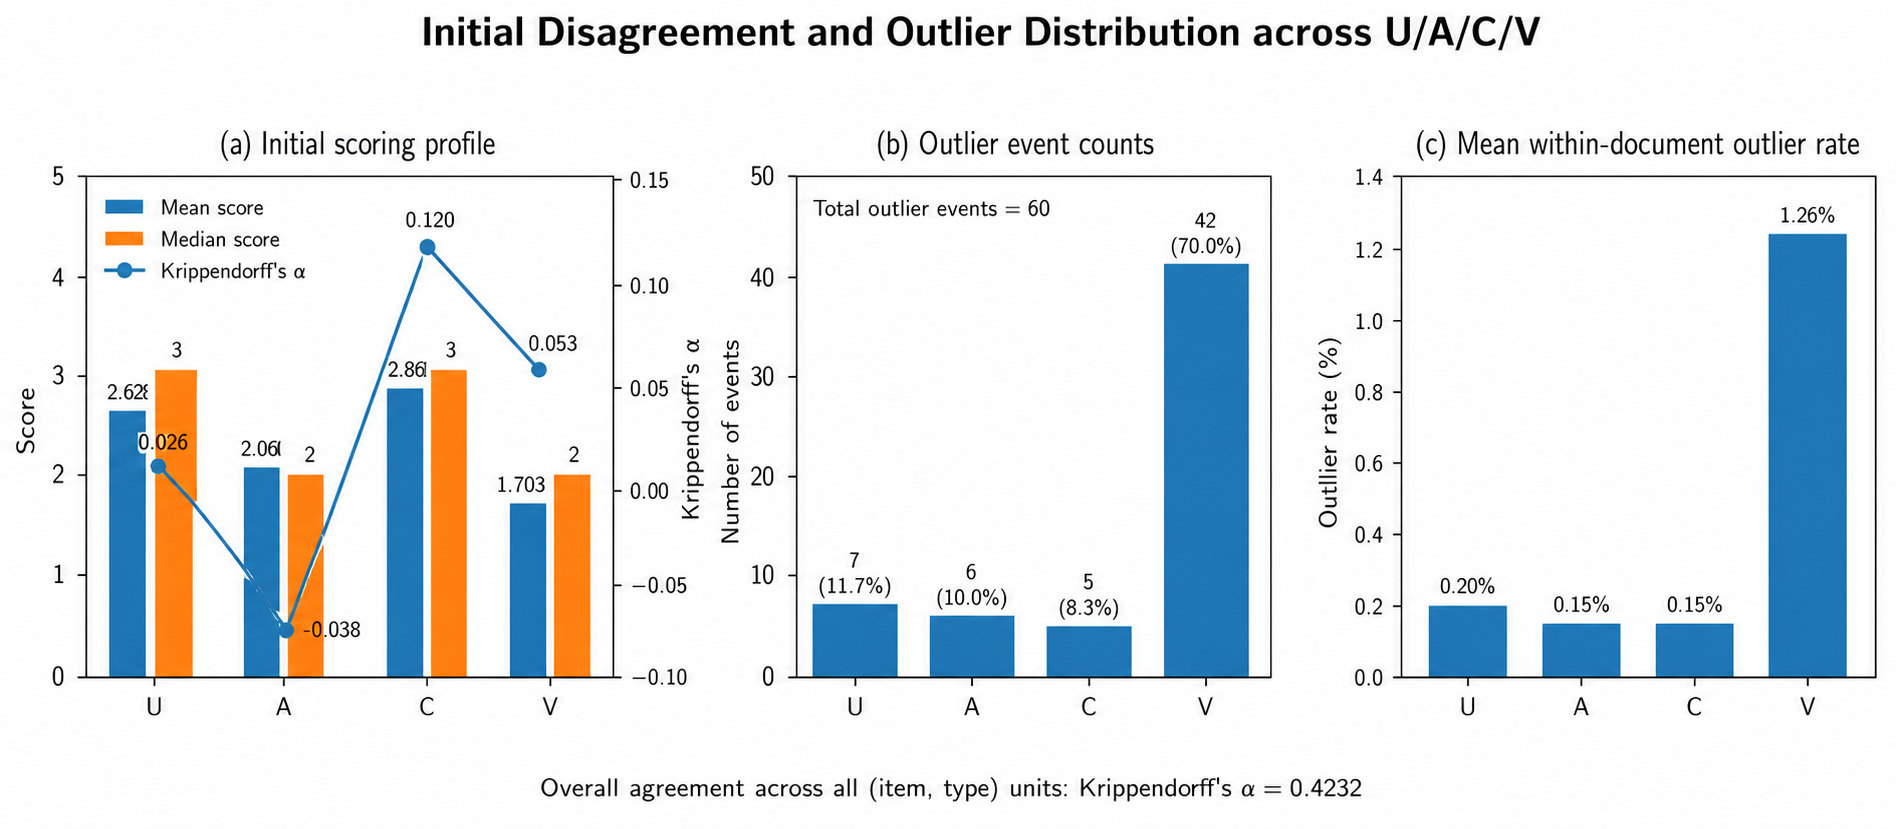
\includegraphics[width=\linewidth]{figures/fig2_rq1_disagreement.png}
\caption{Initial disagreement and outlier distribution across U/A/C/V.}
\label{fig:rq1_disagreement}
\end{figure}

\noindent\textit{Result for RQ1:} individual LLMs do not merely produce unstructured noise; they exhibit observable structural differences in score level, dimension sensitivity, and where strong disagreement is triggered. V in particular has the lowest mean and the most concentrated outliers, providing a solid empirical basis for treating model disagreement as an exploitable structured signal.

\subsection{RQ2: How does the proposed workflow compare with individual LLMs and aggregation baselines?}
RQ2 evaluates the proposed outlier-aware consensus workflow against single-model, equal-weight, and unweighted-roundtable baselines. To avoid attributing overall changes to any single component, we report, in order, outlier-quality discrimination, treatment-level GT alignment, model-profiling/weighting ablation, and roundtable convergence and issue-list size.

\subsubsection{Good and bad outlier separation}
After argument-quality scoring and decision over the 60 outlier events, the current rules yield 26 \texttt{good}, 15 \texttt{bad}, and 19 \texttt{uncertain}. The overall hard-fail rate is $21.67\%$, and $100.00\%$ of hard-fail events end up \texttt{bad}, confirming that this floor rule effectively intercepts low-quality deviation. The argument-quality score shows clear stratification: \texttt{good} events have median $0.7500$ (mean $0.7788$); \texttt{bad} events median $0.2500$ (mean $0.3056$); \texttt{uncertain} in between (median $0.4167$, mean $0.4386$). Mann--Whitney U tests show a significant difference between \texttt{good} and \texttt{bad} ($p<0.05$); merging \texttt{bad} and \texttt{uncertain} into \texttt{non-good}, \texttt{good} vs.\ \texttt{non-good} is also significant ($p<0.05$). The discrimination thus relies not on ``large deviation'' alone but on textual evidence depth, effectively separating high-value dissent from low-quality deviation.

\begin{figure}[t]
\centering
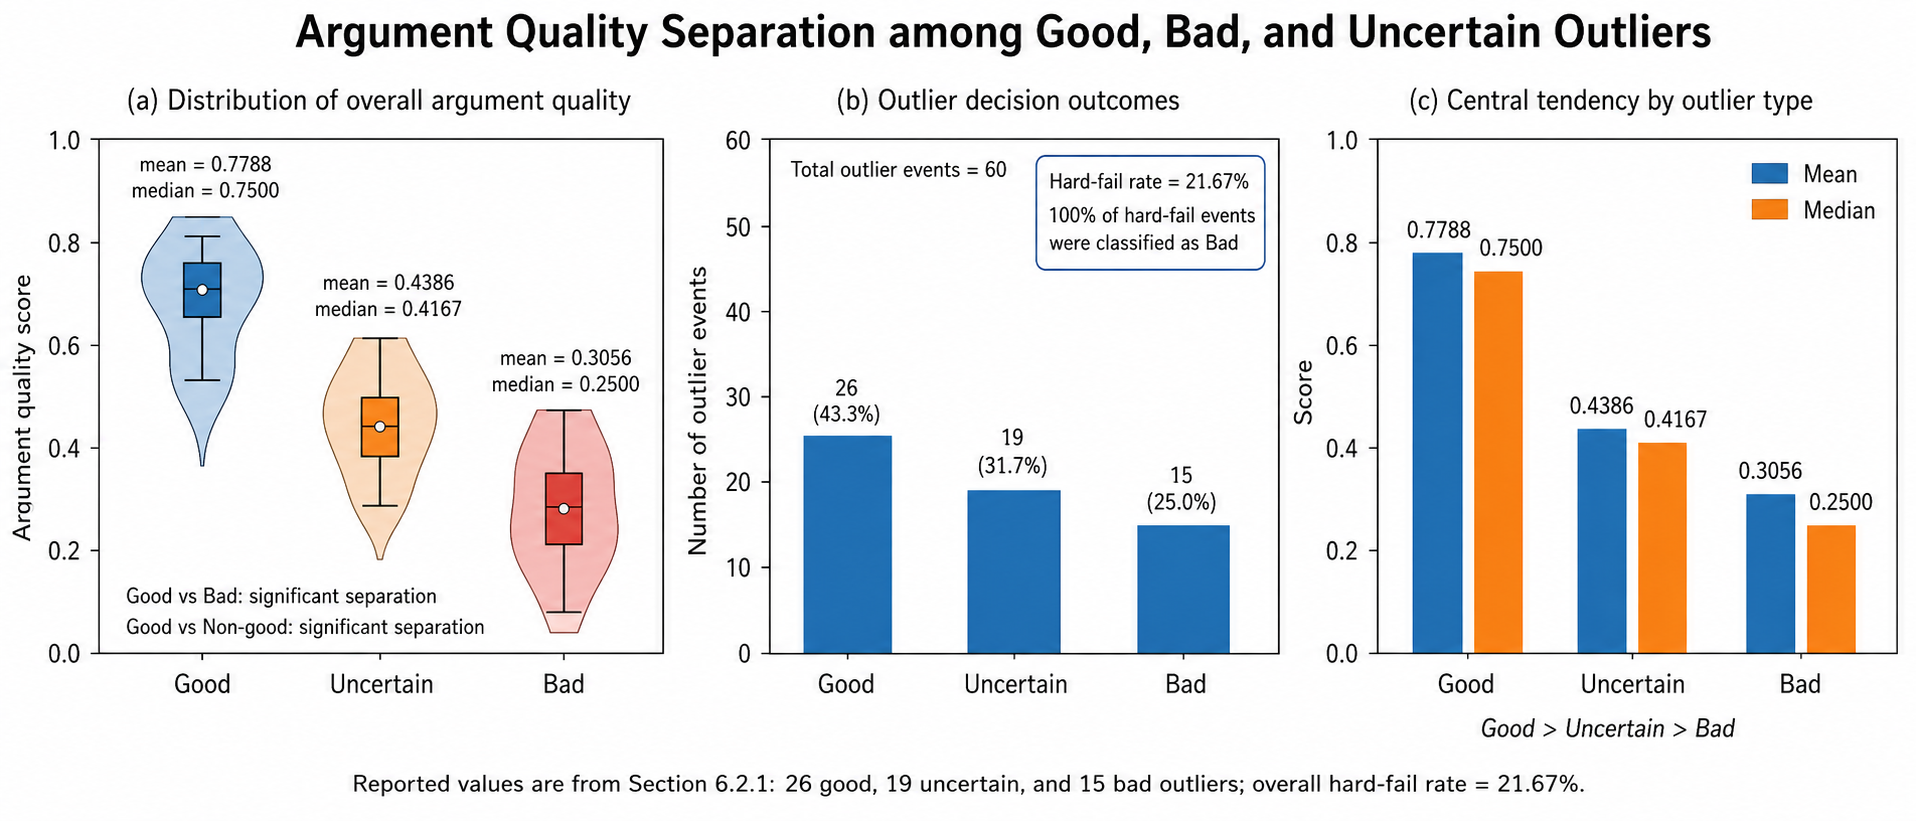
\includegraphics[width=\linewidth]{figures/fig3_outlier_separation.png}
\caption{Argument-quality separation among good, bad, and uncertain outliers.}
\label{fig:outlier_separation}
\end{figure}

\subsubsection{Treatment-level performance}
\begin{sidewaystable}
\centering
\caption{Treatment-level performance results.}
\label{tab:treatment_results}
\footnotesize
\renewcommand{\arraystretch}{1.2}
\begin{tabular}{p{3.2cm}cccp{2.2cm}p{4.6cm}p{3.0cm}}
\toprule
\textbf{Treatment} & \textbf{Macro-P} & \textbf{Macro-R} & \textbf{Macro-F1} & \textbf{Avg.\ pred.\ issues} & \textbf{Primary characteristic} & \textbf{Role} \\
\midrule
Single-LLM Family Mean & 0.0769 & --- & 0.0960 & --- & Balanced single-model behaviour & Reference \\
Equal-Weight Aggregation & 0.0771 & 0.4077 & \textbf{0.1153} & 144.8 & Highest recall; very large list & Aggregation baseline \\
Roundtable No Weighting & --- & --- & 0.0968 & 136.7 & Consensus without reliability weighting & Ablation \\
Full Method & \textbf{0.0901} & 0.1354 & 0.0711 & \textbf{15.9} & Highest precision; strongest compression & Proposed \\
\bottomrule
\end{tabular}

\par\vspace{0.4em}
{\footnotesize \textit{Overall comparison.} A Friedman test on document-level Macro-F1 finds no statistically significant overall difference among the four treatments ($\chi^2=2.0400$, $p=0.5641$, Kendall's $W=0.0680$). Although the Full Method does not achieve the highest Macro-F1, it produces substantially more compact issue lists while improving precision, indicating a selective issue-generation strategy rather than a high-recall detector. \textit{Note.} Macro-P = Macro-Precision; Macro-R = Macro-Recall. Values are averaged over the 10 shared requirements documents. ``---'' denotes values not emphasized in the current study.\par}
\end{sidewaystable}

Under strict paired comparison over the 10 shared documents, document-level Macro-F1 means differ somewhat: Equal-Weight Aggregation is highest ($0.1153$), followed by Roundtable No Weighting ($0.0968$) and Single-LLM Family Mean ($0.0960$), with Full Method lowest ($0.0711$). However, a Friedman test finds no statistically significant overall difference ($\chi^2=2.0400$, $p=0.5641$, Kendall's $W=0.0680$), indicating a small effect size; thus no method holds a stable advantage on document-level Macro-F1.

A likely reason is that the Full Method is not designed to maximize average score or label overlap, but to produce a more reviewable issue list via outlier recognition, profiling, and dynamic confidence. Its Precision/Recall profile shows a selective-output tendency: Macro-Precision $0.0901$ exceeds Equal-Weight's $0.0771$ and Single-LLM's $0.0769$, while Macro-Recall is only $0.1354$, well below Equal-Weight's $0.4077$. Correspondingly, the Full Method outputs only $15.9$ issues per document on average versus Equal-Weight's $144.8$. Hence the Full Method is not a high-recall detector but a more compact, higher-precision, more selective issue-list generator.

\subsubsection{Model profiling and fixed weighting (ablation)}
\begin{table}[t]
\centering
\caption{Model profiling and fixed weighting.}
\label{tab:model_profile_weights}
\small
\begin{tabular}{lc}
\toprule
\textbf{Model} & \textbf{Avg.\ fixed weight} \\
\midrule
DeepSeek & 0.3129 \\
GPT      & 0.2738 \\
Kimi     & 0.2732 \\
Qwen     & 0.2598 \\
GLM-5    & 0.1437 \\
\bottomrule
\end{tabular}

\vspace{0.4em}
\begin{minipage}{0.95\linewidth}
\footnotesize
\textit{Note.} Average document-level fixed weights derived from good-/bad-outlier evidence. The average fixed weight is strongly negatively correlated with each model's single-model Macro-Recall and Macro-F1 (Spearman $\rho=-0.80$ and $-0.90$, respectively), indicating that the weight reflects a model's contribution to capturing high-value outliers rather than its standalone classification ability. Ablation: replacing profiling weights with equal weights changes Macro-F1 only marginally (Full Method $0.0711$ vs.\ equal-weight variant $0.0704$; Wilcoxon paired test $p=0.7500$), while the average number of predicted issues decreases from $17.6$ to $15.9$.
\end{minipage}
\end{table}

The five models' average fixed weights are DeepSeek ($0.3129$), GPT ($0.2738$), Kimi ($0.2732$), Qwen ($0.2598$), and GLM-5 ($0.1437$). Notably, the average fixed weight is strongly negatively correlated with a model's single-model Macro-Recall and Macro-F1 ($-0.8000$ and $-0.9000$), confirming that the weight is not a static ranking of overall classification ability but a dynamic measure of a model's contribution to capturing high-value outliers in the current document. The \texttt{full\_method\_equal\_weights} ablation (replacing profile weights with equal weights) further quantifies the module: Full Method ($0.0711$) and the equal-weight variant ($0.0704$) have nearly identical Macro-F1 (Wilcoxon paired test $p=0.7500$), the only difference being that profile weights reduce the average predicted issues from $17.6$ to $15.9$. Thus the main observable effect comes from the combination of outlier-aware filtering, issue-set convergence, and final list compression, not from directly raising macro classification metrics.

\subsubsection{Roundtable convergence and issue-list compactness}
The roundtable shows very strong set-level convergence. Comparing Full Method with Roundtable No Weighting over the 10 documents: the Full Method's issue-convergence success rate (\texttt{issue\_converged}) reaches $100.00\%$, with a final-round average issue-set Jaccard of $0.9838$ and an average final maximum score difference (\texttt{max\_score\_diff}) of $0.7819$; Roundtable No Weighting reaches $90.00\%$, with final Jaccard $90.02\%$ and max score difference $1.1789$. The score-convergence rate is $0.00\%$ for all methods, showing that issue-set agreement precedes numeric-score agreement. In terms of list size, the Full Method compresses 611 initial candidates to 159 final issues over the 10 documents (retention $26.02\%$); under the same scope the average predicted issues are $15.9$ (Full Method), $136.7$ (Roundtable No Weighting), and $144.8$ (Equal-Weight). The workflow thus greatly reduces final output size and forms a more stable issue set, improving compactness and engineering actionability.

\begin{figure}[t]
\centering
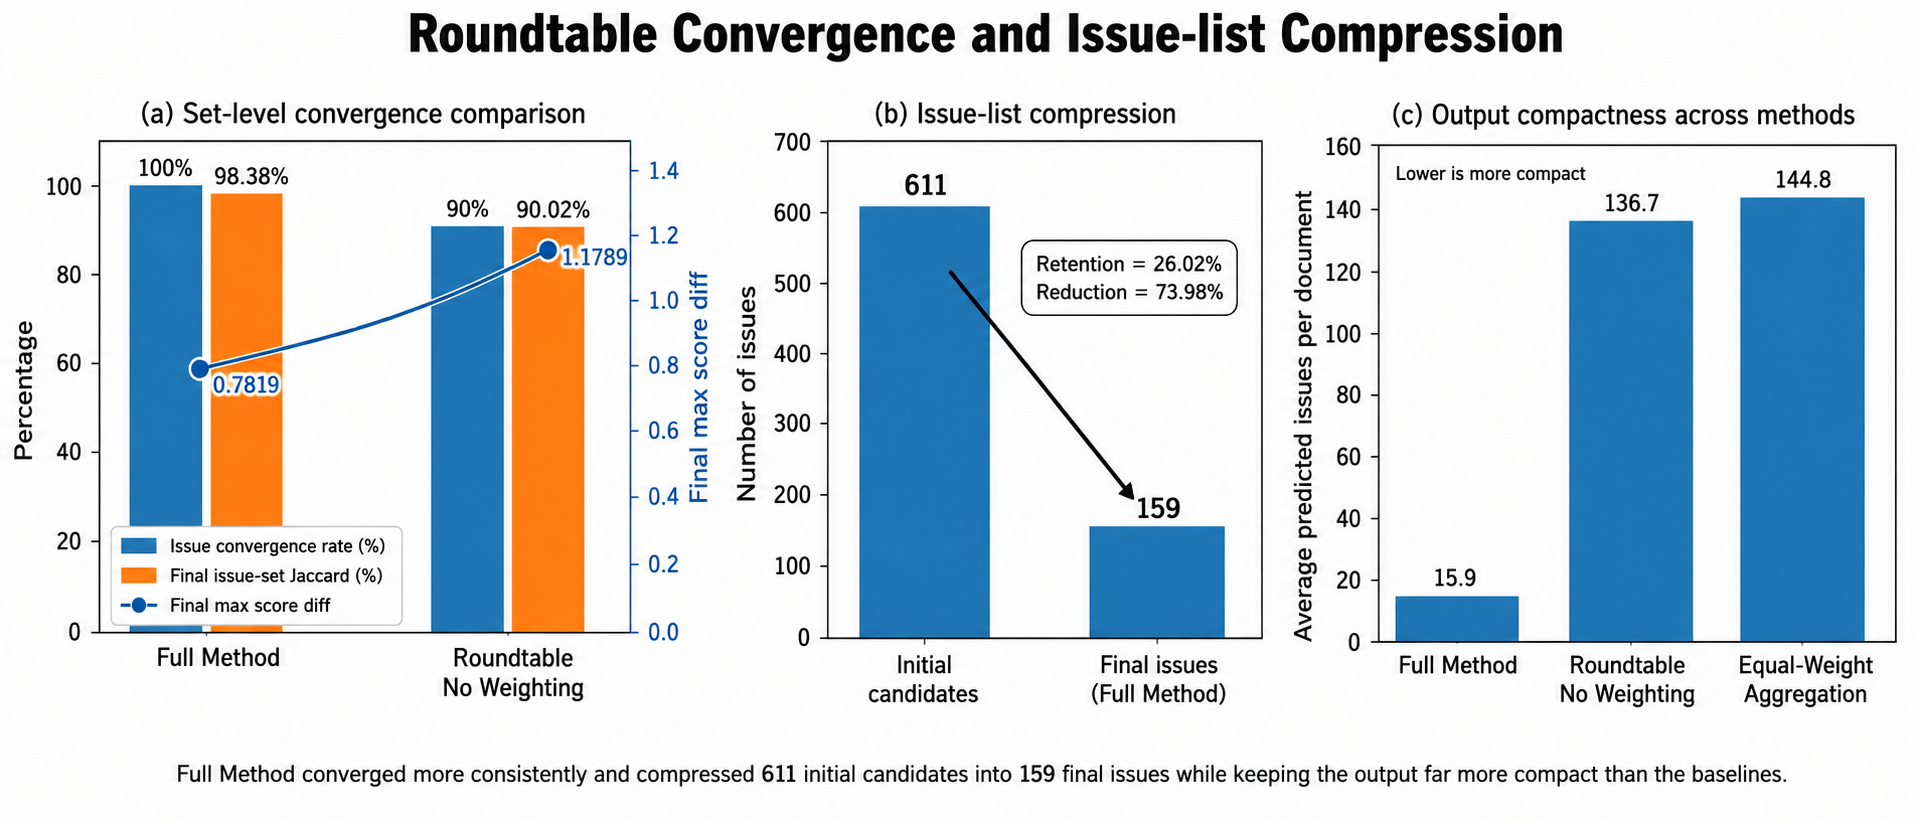
\includegraphics[width=\linewidth]{figures/fig4_convergence.png}
\caption{Roundtable convergence and issue-list compression.}
\label{fig:convergence}
\end{figure}

\noindent\textit{Result for RQ2:} the workflow does not uniformly outperform baselines on all traditional metrics; rather it exhibits a clear trade-off. It effectively discriminates dissent quality and yields a compact, highly stable, higher-precision issue list, at the cost of recall. The ablation shows the marginal utility of profile weighting lies in strengthening candidate compression rather than raising F1.

\subsection{RQ3: How does the workflow vary across documents and quality dimensions?}
The Full Method's performance shows clear document heterogeneity and dimensional preference. \textbf{Document level}: on documents with dense initial candidates it yields sizable F1 gains---e.g., \texttt{2005 - phin} (200 initial issues compressed to 10) improves Macro-F1 from $0.0859$ to $0.1667$, and \texttt{2007 - puget sound} from $0.1498$ to $0.1867$---but these gains come mainly from precision improvements due to redundancy filtering, inevitably accompanied by recall loss. \textbf{Dimension level}: on de-duplicated $(item,type)$ candidates, the initial list is fairly balanced across U/A/C/V ($\approx 25\%$, $26\%$, $20\%$, $29\%$), but after the full pipeline the final list shifts drastically to $1.26\%$, $39.62\%$, $0.00\%$, and $59.12\%$. The system strongly favors retaining Verifiability (V) and Unambiguity (A) issues.

\begin{figure}[t]
\centering
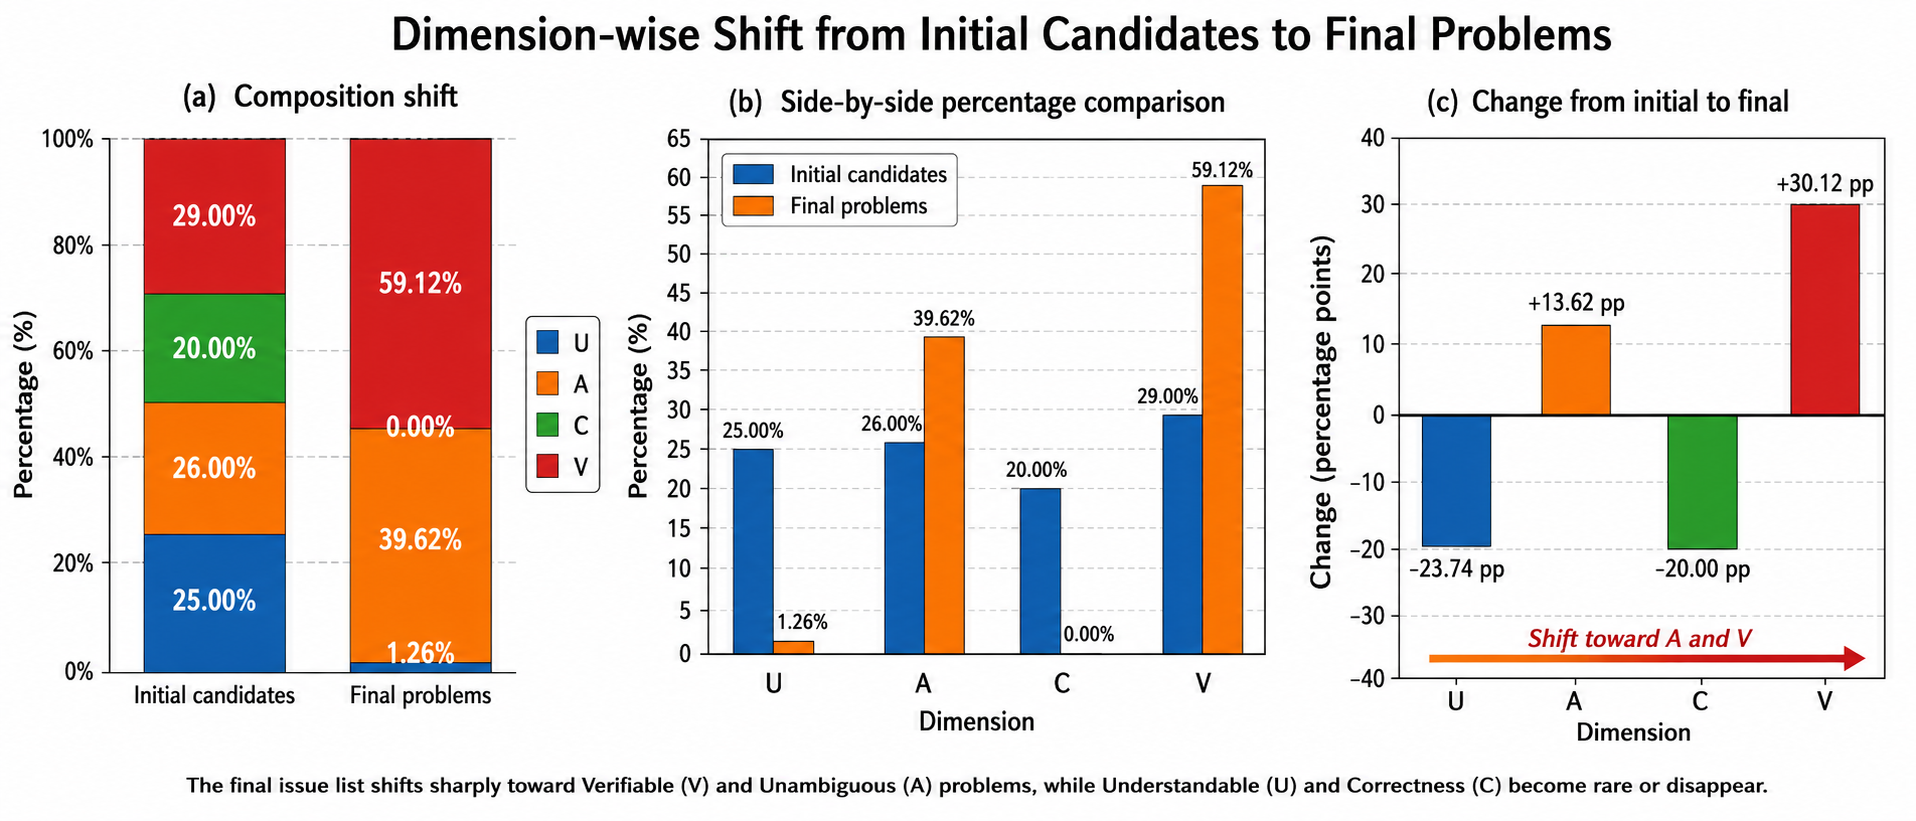
\includegraphics[width=\linewidth]{figures/fig5_dimension_shift.png}
\caption{Dimension-wise shift from initial candidates to final problems.}
\label{fig:dimension_shift}
\end{figure}

\noindent\textit{Result for RQ3:} the workflow is highly context-dependent. On documents with dense candidates its pruning best translates into precision gains, and its final output concentrates on V and A defects, reflecting that model interaction reaches rational consensus more easily on such formally/semantically well-bounded tasks.

\subsection{Summary of findings}
(1) \textbf{Structural disagreement exists}: LLMs do not produce random noise in per-requirement quality identification but show significant structural outlier concentration, notably on V. (2) \textbf{Trade-off performance profile}: the workflow separates good/bad outliers and yields a compact, higher-precision, highly stable expert-level issue list, but cannot statistically avoid a marked recall loss. (3) \textbf{Bounded role of weighting}: fixed weighting via model profiling mainly smooths and compresses redundant candidates rather than creating a significant Macro-F1 gain. (4) \textbf{Generalization heterogeneity}: the advantage concentrates on denoising candidate-dense documents, with the final output strongly biased toward V and A.

\section{Validity Threats and Discussion}\label{sec:validity}
\subsection{Validity threats}
\subsubsection{Construct validity}
Construct validity concerns the match between theoretical concepts and actual metrics. The core threat is the definition of the argument-quality score $Q$, the six features, and the hard-fail rule, whose rules and empirical thresholds may carry subjective bias. \textit{Mitigation:} our dimension definitions (U/A/C/V) map strictly onto classic IEEE requirements-specification standards and established empirical-SE taxonomies; for $Q$, we avoid complex non-linear weighting and instead use simple uniform normalization plus a hard-fail floor, reducing overfitting risk. The ablation (unweighted roundtable vs.\ full method) further shows that the current settings produce meaningful discrimination in practice.

\subsubsection{Internal validity}
Internal validity concerns implementation details that may confound causal relations. The main threat is the instability of real API services: rate limiting, timeouts, or malformed JSON can cause some models to be skipped on specific items, so the effective number of models per document/item is not perfectly uniform. Additionally, current parameters (outlier threshold, good/bad thresholds, penalty coefficient, Top-$K$, and maximum rounds) are set empirically. \textit{Mitigation:} we explicitly treat API instability as part of robustness: a retry and case-level isolation mechanism disables a model only on the failing item while others continue; results are aggregated at document-level Macro-F1, diluting the random impact of individual lost requests.

\subsubsection{External validity}
External validity concerns generalization to other settings or future models. First, although PURE is real, it mainly represents traditional SRS documents and may not extend directly to highly agile user stories or specific regulated domains; second, the five chosen LLMs are time-sensitive. \textit{Mitigation:} we sample documents across domains, sizes, and defect densities; at the model level we validate the methodology of value-discriminated dynamic weighting and roundtable rather than a permanent ranking of specific models, and the framework is in principle decoupled from the underlying models.

\subsubsection{Conclusion validity}
Conclusion validity concerns whether the statistical analysis supports the inferences. The main threat is statistical bias from document heterogeneity (large differences in size and defect density); mixing all items to compute $p$-values risks Simpson's paradox. \textit{Mitigation:} we strictly use ``document'' as the paired-comparison block, apply robust non-parametric tests (Friedman and paired Wilcoxon signed-rank), and mandatorily report non-parametric effect sizes (Cliff's $\delta$).

\subsection{Discussion}
\begin{table}[t]
\centering
\caption{Representative good and bad outlier cases.}
\label{tab:representative_outlier_cases}
\renewcommand{\arraystretch}{1.15}
\resizebox{\textwidth}{!}{%
\begin{tabular}{p{1.0cm}p{1.6cm}p{0.8cm}p{1.4cm}p{1.2cm}p{2.8cm}p{3.1cm}p{3.2cm}}
\toprule
\textbf{Case} & \textbf{Item} & \textbf{Type} & \textbf{Score / Median} & \textbf{Decision} & \textbf{Requirement excerpt} & \textbf{Model evidence} & \textbf{Adjudication rationale} \\
\midrule
G1 & \texttt{[doc--item]} & V & \texttt{[score]/[median]} & Good & \textit{``[short requirement excerpt]''} & \textit{``[evidence span]''} & Retained: the model identifies a concrete verifiability problem, gives a traceable textual cue, and proposes a testable or measurable revision. \\
\midrule
G2 & \texttt{[doc--item]} & A & \texttt{[score]/[median]} & Good & \textit{``[short requirement excerpt]''} & \textit{``[evidence span]''} & Retained: the minority judgment exposes an ambiguity missed by the group median, while the evidence and rewrite remain dimension-aligned and actionable. \\
\midrule
B1 & \texttt{[doc--item]} & U & \texttt{[score]/[median]} & Bad & \textit{``[short requirement excerpt]''} & \textit{``[evidence span]''} & Rejected: the explanation is weak or generic and does not clearly identify a textual defect, failing to justify the large deviation. \\
\midrule
B2 & \texttt{[doc--item]} & C & \texttt{[score]/[median]} & Bad & \textit{``[short requirement excerpt]''} & \textit{``[evidence span]''} & Rejected: reflects a dimension mismatch or an unsupported correctness claim rather than a demonstrable defect. \\
\bottomrule
\end{tabular}%
}

\vspace{0.4em}
\begin{minipage}{0.97\textwidth}
\footnotesize
\textit{Note.} Good outliers are minority judgments that deviate from the group median but provide sufficient evidence, dimension-aligned reasoning, and executable rewrite suggestions. Bad outliers are deviations rejected by the argument-quality assessment or hard-fail rules (missing evidence, non-executable rewrites, or dimension mismatch). Bracketed placeholders should be replaced with real cases; complete cases are provided in the replication package.
\end{minipage}
\end{table}

Three insights stand out. First, in multi-LLM requirements review, ``minority opinions'' are not noise to be erased but a potential information source to be examined further; what matters is not whether a judgment deviates from consensus, but whether the deviation is backed by high-quality evidence and an executable rewrite. Second, model weighting should be understood not as a static ranking of ability but as a document-internal, task-internal, evidence-driven trust allocation. Third, the main value of roundtable consensus is not to make numeric scores identical but to help the system converge, within a few rounds, to a more compact and actionable issue set. Overall, the results support the feasibility of our ``from disagreement to consensus'' framework, while the validity threats indicate that it should be viewed as a promising method requiring further validation in larger controlled studies.

\FloatBarrier
\section{Conclusion}\label{sec:conclusion}
The integration of multiple LLMs in software engineering has long been constrained by the majority-vote assumption of ``convergence implies correctness'', which tends to erase high-value minority opinions through group smoothing. Against this consensus fallacy, we build a heterogeneous multi-model roundtable-consensus framework for per-requirement quality assessment. By introducing an outlier-discrimination mechanism grounded in textual argumentation, the framework converts structured inter-model disagreement into global trust weights and, over multiple rounds, fuses these static weights with dynamic confidence to drive rational team consensus.

Empirically, our results establish a key shift in automated requirements review: in complex engineering reasoning, score disagreement is itself a highly discriminative signal. Using an argument-quality vector built from evidence sufficiency and rewrite executability, the system penetrates numerical deviation, blocks unsupported hallucinations (bad outliers), and amplifies well-reasoned minority insights (good outliers). Compared with equal-weight ensembling, weighting and roundtabling based on outlier history achieve rapid convergence of the defect set within limited rounds. Future work can (i) extend the framework to more context-dependent artifacts such as agile user stories and architecture design documents; (ii) add explicit cross-item consistency checks and external domain-knowledge constraints to the argument-quality vector to better capture hidden correctness defects; and (iii) explore finer-grained local fault tolerance and model substitution under highly heterogeneous or edge-deployment settings toward industrial-grade automated quality-assurance pipelines.

\backmatter

\bmhead{Data Availability Statement}
The PURE dataset used in this study is publicly available. The requirement subsets, prompts, model outputs, ground-truth annotations, and analysis scripts that support the findings are available in the replication package (to be released upon acceptance / from the corresponding author on reasonable request).

\bmhead{Declarations}
The authors declare no competing interests relevant to this article. (Competing interests, author contributions, and funding are submitted via the journal system and the separate title page in accordance with the double-anonymous policy.)

\bibliography{references}

\end{document}
